\documentclass{ctexart}
\textheight 23.5cm \textwidth 15.8cm
\topmargin -1.5cm \oddsidemargin 0.3cm \evensidemargin -0.3cm

\usepackage{verbatim}
\usepackage{fancyhdr}
\usepackage{float}
\usepackage{graphicx}
\usepackage{amssymb}
\usepackage{amsmath}


\pagestyle{fancy}
\CTEXsetup[format = {\Large\bfseries\it}]{section}


\begin{document}

\section*{内容简介}
	\noindent 初值问题
	\begin{equation}
	\left\{\begin{aligned}
		& y' = \dfrac{x − e^{−x}}{y + e^y}\\
		& y(0) = 0
	\end{aligned}\right.
	\end{equation}
	该方程的真解由等式
	\begin{equation}
		y^2 − x^2 + 2e^y − 2e^{−x} = 0
	\end{equation}
	隐式给出。
	\begin{itemize}
		\item 当 $x = 1$ 时,数值求解等式
		\begin{equation*}
			y^2 − x^2 + 2e^y − 2e^{−x} = 0
		\end{equation*}
		将这一数值解作为参考的准确解。
		
		\item 利用五阶 Adams-Bashforth 公式计算方程在 $x = 1$ 的数值解。用五阶 Runge-Kutta 格式得到初值,取节点 $x_i$,$i = 0,\cdots,N$,$N$ 为 $2^k$,$k = 3,\cdots, 8$,给出误差表格,其中阶为
		\begin{equation}
			\dfrac{\ln(Error_{old} / Error_{now})}{\ln(N_{now} / N_{old})}		
		\end{equation}
	\end{itemize}
	
	
\section*{工作环境}
	程序所用语言: {\bf python}
	
	软件: {\bf JupyterLab}
	
	使用的包: {\bf numpy,scipy.optimize,mpmath }

\section*{输出结果}

\begin{verbatim}
	EQN:
	f(x, y) = (x - e^(-x)) / (y + e^y)
	y(0) = 0
	Real : y1(1.000000) = -1.000000000000
	
	Adams-Bashforth :
	[k = 3]  y(1.000000) = -1.000000000000, Error = 4.463096558993e-14, Order = -inf
	[k = 4]  y(1.000000) = -1.000000000000, Error = 0.000000000000e+00 // Max precision reached
	[k = 5]  y(1.000000) = -1.000000000000, Error = 0.000000000000e+00 // Max precision reached
	[k = 6]  y(1.000000) = -1.000000000000, Error = 0.000000000000e+00 // Max precision reached
	[k = 7]  y(1.000000) = -1.000000000000, Error = 0.000000000000e+00 // Max precision reached
	[k = 8]  y(1.000000) = -1.000000000000, Error = 0.000000000000e+00 // Max precision reached
\end{verbatim}
	因 $k = 4$ 以后在该浮点数精度下已与准确解相等,打印精度检验表是没有意义的。
	
\section*{分析}
	\subsection*{一、Adams-Bashforth 公式}
		\noindent Adams-Bashforth 公式(下简记为 A-B 公式)的形式为
		\begin{equation}
			y_{n+1} = y_{n} + a_0 f_{n} + a_1 f_{n-1} + a_2 f_{n-2} + \cdots
		\end{equation}
		
		\noindent 其中 $f_{i}$ 表示 $f(x_i,\,y_i)$。
		
		基于等距结点的五阶 A-B 公式为
		\begin{equation}
			y_{n+1} = y_{n} + \dfrac{h}{720}\left[ 1901 f_{n} - 2774 f_{n-1} + 2616 f_{n-2} - 1274 f_{n-3} + 251f_{n-4} \right]
		\end{equation}
		
		\noindent 定义线性泛函
		\begin{align*}
			L(y) & = \sum_{i = 0}^5 \left[ a_i y_i - h b_i y_i'\right] \\
			& = y_5
			+ \left[ - y_4 - \dfrac{1901}{720} h f_4 \right]
			+ \left[ \dfrac{1387}{720} h f_3 \right]
			+ \left[ - \dfrac{77}{90} h f_2 \right]
			+ \left[ \dfrac{637}{360} h f_1 \right]
			+ \left[ - \dfrac{251}{720} h f_0 \right]
		\end{align*}
		其中
		\begin{equation}
		\begin{cases}
		\displaystyle
		a_0 = a_1 = a_2 = a_3 = 0\\
		a_4 = -1,\quad a_5 = 1 \\
		b_0 = - \frac{251}{720},\quad b_1 = \frac{637}{360} \\
		b_2 = - \frac{77}{90},\quad b_3 = \frac{1387}{720} \\
		b_4 = \frac{1901}{720},\quad b_5 = 0
		\end{cases}
		\end{equation}
		
		利用 Taylor 级数,$L(y)$ 也可表示为
		\begin{equation}
			L(y) = d_0 y_0 + d_1 h y_1' + d_2 h^2 y_2'' + \cdots
		\end{equation}
		比较两式,从而计算出
		\begin{equation}
		\begin{cases}
			\displaystyle d_0 = \sum_{i = 0}^5 a_i = 0 \\
			\displaystyle d_1 = \sum_{i = 0}^5 (i a_i - b_i) = 0 \\
			\qquad \cdots\\
			\displaystyle d_5 = \sum_{i = 0}^5 \left(\frac{i^5}{120} a_i - \frac{i^4}{24} b_i \right) = 0 \\
			\displaystyle d_6 = \sum_{i = 0}^6 \left(\frac{i^6}{720} a_i - \frac{i^5}{120} b_i \right) \neq 0
		\end{cases}
		\end{equation}
		
		根据 [1,\,p447] 多步法局部截断误差定理,五阶 A-B 方法的局部截断误差为 $O(h^6)$。再由 [1,\,p448] 整体误差截断定理知 五阶 A-B 方法的整体截断误差为 $O(h^5)$。
		
		与该方法稳定性和相容性相关的两个多项式为
		\begin{equation}
		\begin{cases}
			p(z) = z^5 - z^4 \\
			q(z) = \dfrac{1}{720}\left[ 1901 z^4 - 2774 z^3 + 2616 z^2 - 1274 z + 251 \right] \\
		\end{cases}
		\end{equation}
		
		多项式 $p$ 的根为 $1$,$0$(四重),因此是稳定的;$q(1) = \dfrac{1}{720}(1901 - 2774 + 2616 - 1274 + 251) = 1$,\\[0.8mm]
		$p(1) = 0$,$p'(1) = 1$,因此也是相容的。根据 [1,\,p446] 多步法稳定性和相容性定理,五阶 A-B 方法是收敛的。
		
		
	\subsection*{二、得到原方程精确解的原因}
		事实上对于原问题,凡是满足形式 $y(x_0) = - x_0$ 的初值条件,根据方程:
		\begin{equation}
			y' = f(x,\,y) = \dfrac{x − e^{−x}}{y + e^y}
		\end{equation}
		
		\noindent 使用五阶 Runge-Kutta 方法计算启动点时,将发生如下现象:从直线 $y = -x$ 上一点 $(x_n,\,y_n)$ 开始计算的下一点
		\begin{align*}
			F_i & = -h\\
			y_{n+1} & = y(x_n + h) = y(x) + \sum_{i = 0}^{6} c_i F_i \\
				& = - (x_n + h) = x_{n+1}
		\end{align*}
		仍落在直线 $y = -x$ 上。因此用于启动五阶 A-B 方法的五个初始点将全部位于这条直线上。
		
		使用 A-B 方法计算时,每次步进 $y_n$ 都将随 $x_n$ 以斜率 $-1$ 线性增长,后续点的数值解都将落在直线 $y = -x$ 上,并最终准确地到达 $(1,\,-1)$,即方程的隐式解在 $x = 1$ 处对应的一个解。可参考下面绘制的向量场。
		
		\begin{figure}[H]
			\centering
			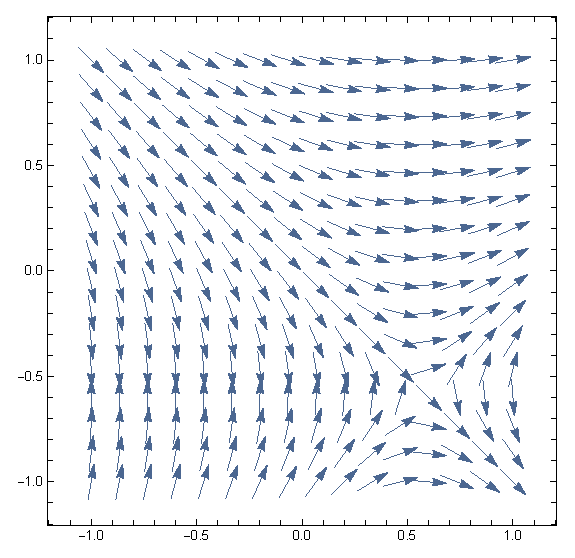
\includegraphics[width = 7cm, height = 7cm]{contour.eps}
			\caption{微分方程向量场} \label{figure.label}
		\end{figure}
		
		进而,$k = 3$ 时误差产生原因可能是由于二进制数不能有限表示某些十进制数、$e$ 指数运算精度有限和一些舍入误差所导致的,并不是方法带来的。
		
		
	\subsection*{三、重新尝试}
	\noindent 尝试对另一个初值问题作相同的工作。选取第 10 次程序作业中的微分方程:
	\begin{equation}
	\left\{\begin{aligned}
		& y' = \lambda y + \cos x - \lambda \sin x\\
		& y(0) = 0
	\end{aligned}\right.
	\end{equation}
	该方程的真解为
	\begin{equation}
		y(x) = \sin x
	\end{equation}
	
	取 $\lambda = 1$,此时利用五阶 Adams-Bashforth 公式计算方程在 $x = 1$ 的数值解,用五阶 Runge-Kutta 格式得到初值,节点选取与原题相同。得到如下结果与误差表格。
	\begin{verbatim}
		EQN:
		f(x, y) = y + cos(x) - sin(x)
		y(0) = 0
		Real : y2(1.000000) = 0.841470984808
		
		Adams-Bashforth :
		[k = 3]  y(1.000000) = 0.841473918590, Error = 2.933781801051e-06, Order = -inf
		[k = 4]  y(1.000000) = 0.841471134292, Error = 1.494840289329e-07, Order = 4.2947
		[k = 5]  y(1.000000) = 0.841470990425, Error = 5.617588283435e-09, Order = 4.7339
		[k = 6]  y(1.000000) = 0.841470984998, Error = 1.904448820866e-10, Order = 4.8825
		[k = 7]  y(1.000000) = 0.841470984814, Error = 6.183387135650e-12, Order = 4.9448
		[k = 8]  y(1.000000) = 0.841470984808, Error = 1.959543638463e-13, Order = 4.9798
	\end{verbatim}
	
	\begin{table}[htb]
		\centering
		\bigskip
		\begin{small}
			\begin{tabular}{|c|cc|}
				\hline
					k & Error & Order\\
				\hline
					3 & 2.9338E-06 & -- \\
					4 & 1.4948E-07 & 4.2947 \\
					5 & 5.6176E-09 & 4.7339 \\
					6 & 1.9044E-10 & 4.8825 \\
					7 & 6.1834E-12 & 4.9448 \\
					8 & 1.9595E-13 & 4.9798 \\
				\hline
			\end{tabular}
		\end{small}
		\caption{\label{table.label} 精度检验}
	\end{table}
	
	五阶 Adams-Bashforth 公式 $O(h^5)$ 的整体截断误差得到了证实。

\section*{参考资料}
	\noindent [1] David R. Kincaid \& E. Ward Cheney. {\it Numerical Analysis: Mathematics of Scientific of Computing Third Edition}, Brooks/Cole, 2002.

\end{document}